\newpage

\subsection{Arcs, sectors and segments}

\begin{theorybox}{}

Using radians, we can deduce other formulae to calculate certain properties of circles and sectors.
\vskip5mm
The arc length, $l$ units, subtended by an angle $\theta$ (radians) in a circle of radius $r$ units is given by $$l=r\theta$$
\begin{center}
    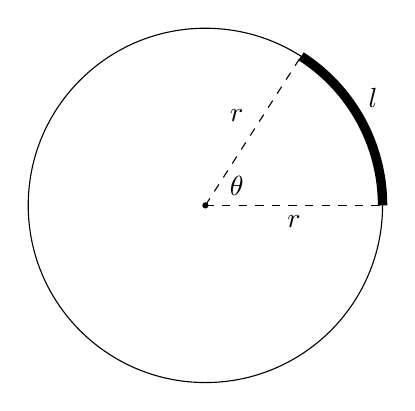
\begin{tikzpicture}[scale=0.75]
        \draw[] (0,0) circle (3cm);
        \fill (0,0) circle (1.5pt);
        \draw[line width=1.2mm] (3,0) arc[start angle=0, end angle=57.2958,radius=3cm];
        \draw [dashed] (0,0) -- node[below]{$r$} (3,0);
        \draw[dashed] (0,0) -- node[above left]{$r$} (1.6209,2.5244);
        \coordinate[label=above right: $l$] (P) at (2.5981, 1.5);
        \coordinate[label=above right: $\theta$] (O) at (0.25,0);
    \end{tikzpicture}
\end{center}

\vskip5mm
The area, $A\ \text{units}^{2}$, of a sector subtended by an angle $\theta$ (radians) in a circle of radius $r$ units is given by $$A=\dfrac{1}{2} r^2 \theta$$
\begin{center}
    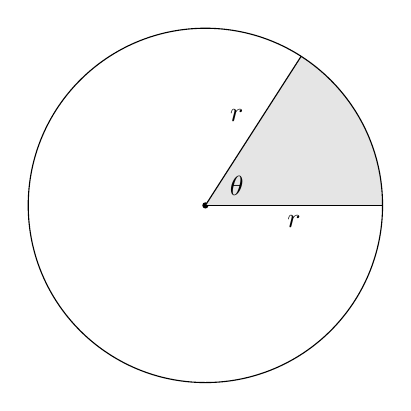
\begin{tikzpicture}[scale=0.75]
        \fill (0,0) circle (1.5pt);
        \fill[color=gray!20!white] (0,0) -- (3,0) arc[start angle=0, end angle=57.2958,radius=3cm] -- (0,0);
        \draw[] (0,0) circle (3cm);
        \draw (0,0) -- node[below]{$r$} (3,0);
        \draw (0,0) -- node[above left]{$r$} (1.6209,2.5244);
        \coordinate[label=above right: $\theta$] (O) at (0.25,0);
    \end{tikzpicture}
\end{center}

\vskip5mm
The area, $A\ \text{units}^{2}$, of a minor segment subtended by an angle $\theta$ (radians) in a circle of radius $r$ units is given by 
$$A=\dfrac{1}{2} r^2 \left( \theta - \sin \theta \right)$$
\begin{center}
    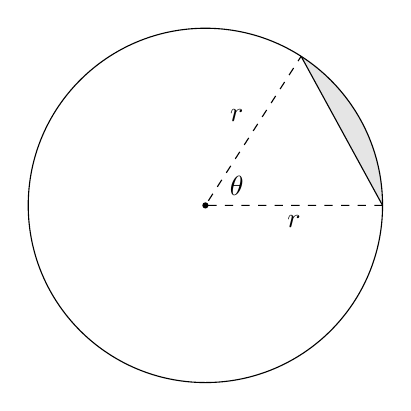
\begin{tikzpicture}[scale=0.75]
        \fill (0,0) circle (1.5pt);
        \fill[color=gray!20!white]  (3,0) arc[start angle=0, end angle=57.2958,radius=3cm] -- (1.6209,2.5244) -- cycle;
        \draw[] (0,0) circle (3cm);
        \draw[dashed] (3,0) -- node[below]{$r$} (0,0) -- node[above left]{$r$} (1.6209,2.5244);
        \draw[] (3,0) -- (1.6209,2.5244);
        \coordinate[label=above right: $\theta$] (O) at (0.25,0);
    \end{tikzpicture}
\end{center}

\end{theorybox}

\newpage

\begin{examplecz}[height fill = true]{}
    A circle centred at $O$ has a radius of $6$\,cm. Points $A$ and $B$ lie on the circumference of the circle such that $\angle AOB = 135^{\circ}$.
    \begin{center}
    \begin{tikzpicture}[]
        \draw[] (0,0) circle (3cm);
        \draw [dashed] (0,0) -- node[below]{$6$\,cm} (3,0) node[right]{$A$};
        \draw[dashed] (0,0) -- (-2.1213, 2.1213) node[above left]{$B$};
        \coordinate[label=below left: $O$] (O) at (0,0);
        \coordinate[] (A) at (3,0);
        \coordinate[] (B) at (-2.1213, 2.1213);
        \tkzLabelAngle[pos=0.7](A,O,B){$135^{\circ}$};
        \fill (0,0) circle (2pt);
    \end{tikzpicture}
\end{center}
    \begin{enumerate}
        \item Find the length of the minor arc $AB$, correct to one decimal place.
        \item Find the area of the sector $OAB$, correct to two decimal places.
    \end{enumerate}
\tcblower
\textbf{Solution:}

\end{examplecz}

\newpage
\begin{examplecz}{}
    The radius of a circle is $3$\,cm and an arc is $0.27\pi$\,cm long. 
    \vskip3mm
    Find the angle subtended at the centre of the circle by the arc, correct to two decimal places.
\tcblower
\textbf{Solution:}
\vspace*{60mm}
    
\end{examplecz}

\vspace*{5mm}
%\begin{examplecz}{}
%    The circumference of a circle is $300$\,mm.
%    \vskip3mm
%    Find the length of the arc that is formed by an angle of $\dfrac{\pi}{6}$ subtended at the centre of the circle.
%\end{examplecz}

%\vspace*{5mm}
%\begin{examplecz}{}
%    Find the angle that is subtended at the centre of the circle by an arc that is $8$\,cm long.
%\end{examplecz}


\begin{examplecz}{}
    The area of the sector of a circle that is subtended by an angle of
    $\dfrac{\pi}{3}$ at the centre is $6\pi\,\text{cm}^2$. 
    \vskip3mm
    Find the radius of the circle.
\tcblower
\textbf{Solution:}
\vspace*{60mm}
\end{examplecz}

%\vspace*{5mm}
%\begin{examplecz}{}
%    A sector of a circle with radius $5$\,cm and an angle of $\dfrac{\pi}{3}$ subtended at the centre is cut out of cardboard. It is then curved around to form a cone.
%    \vskip3mm
%    Find its exact surface area and volume.
%\end{examplecz}

\newpage
\begin{examplecz}{}
    The area of a sector is $\dfrac{3\pi}{10}\,\text{cm}^2$ and the arc length cut off by the sector is $\dfrac{\pi}{5}\,\text{cm}$
    \vskip3mm
    Find the angle subtended at the centre, and the radius, of the circle.
\tcblower
\textbf{Solution:}
\vspace*{60mm}
\end{examplecz}

\vspace*{5mm}
\begin{examplecz}{}
    Find the area of the minor segment formed by an angle of $40^{\circ}$ subtended at the centre of a circle with radius $2.82$\,cm, correct to two significant figures.
\tcblower
\textbf{Solution:}
\vspace*{60mm}
\end{examplecz}

\newpage

\begin{examplecz}{}
    An angle of $\dfrac{\pi}{8}$ is subtended at the centre of a circle. This angle cuts off an arc of $54\pi$\,cm.
    \begin{enumerate}
        \item Find the exact area of the sector.
        \item Find the area of the minor segment formed, correct to 1 decimal place.
    \end{enumerate}
\tcblower
\textbf{Solution:}
\vspace*{80mm}
\end{examplecz}

\newpage


\begin{examplecz}[]{}
    A circular chocolate wafer of radius $2$\,cm is dipped in chocolate so that the length of the straight edge measures $3$\,cm as shown.
    \begin{center}
        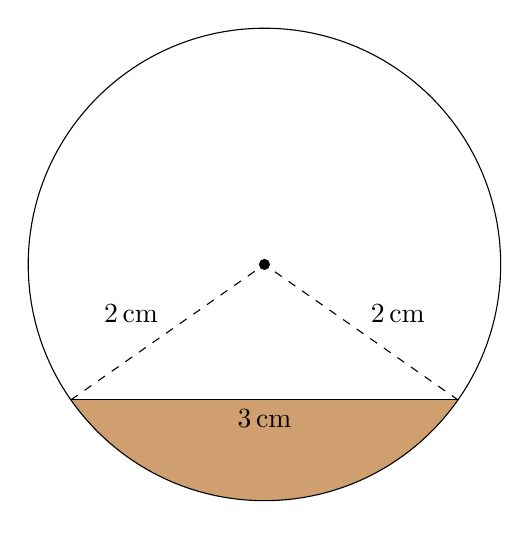
\begin{tikzpicture}[scale=1]
            
            \fill[color=brown!75!white]  (-2.4575,-1.720) arc[start angle=215, end angle=325,radius=3cm] -- (2.4575,-1.720) -- cycle;
            \draw[] (0,0) circle (3cm);
            
            \draw[dashed] (-2.4575,-1.720) -- node[above left]{$2$\,cm} (0,0) -- node[above right]{$2$\,cm} (2.4575,-1.720);
            
            \draw[] (-2.4575,-1.720) -- node[below]{$3$\,cm} (2.4575,-1.720);
            \fill (0,0) circle (2pt);
            
        \end{tikzpicture}
    \end{center}

    Find the area of the wafer that is not covered in chocolate, correct to two decimal places.
    \tcblower
\textbf{Solution:}
\vspace*{100mm}
\end{examplecz}

\begin{comment}
\begin{examplecz}{}
    Point $A$ on a circular wheel of radius $1$ metre sits on a horizontal surface. Point $B$ is lies at an arc length of $2$ metres from $A$ as shown.
    \begin{center}
    \begin{tikzpicture}[]
        \draw[] (0,0) circle (3cm);
        \draw (-4,-3) -- (4,-3);
        \draw[dashed, ->] (-2.3,2.3) arc (135:270:3.25) node[midway,left]{$2$\,m}; angle=270,radius=3.25cm];
        \draw [dashed] (0,0) -- node[right]{$1$\,m} (0,-3) node[below right]{$A$};
        \draw[dashed] (0,0) -- (-2.1213, 2.1213) node[above]{$B$};
        \fill (0,0) circle (2pt) node[above right]{$O$};
        \coordinate[] (A) at (3,0);
        \coordinate[] (B) at (-2.1213, 2.1213);
    \end{tikzpicture}
\end{center}

    \begin{enumerate}
        \item Find the size of $\angle AOB$, correct to three decimal places.
        \item The wheel turns counter-clockwise, without slipping, so that point $B$ rests on the surface.
        \vskip3mm
        Find the vertical height of point $A$ above the ground, correct to one decimal place.
    \end{enumerate}
\end{examplecz}
\end{comment}

\vfill

\begin{Qbox}{}
    From \textit{CambridgeMaths Year 11 Mathematics Extension 1}:
    \begin{itemize}
        \item Exercise 11I: 1 to 16
    \end{itemize}
\end{Qbox}